\documentclass[conference]{IEEEtran}
\IEEEoverridecommandlockouts
% The preceding line is only needed to identify funding in the first footnote. If that is unneeded, please comment it out.
\usepackage{cite}
\usepackage{amsmath,amssymb,amsfonts}
\usepackage{algorithmic}
\usepackage{graphicx}
\usepackage{textcomp}
\usepackage{xcolor}
\def\BibTeX{{\rm B\kern-.05em{\sc i\kern-.025em b}\kern-.08em
    T\kern-.1667em\lower.7ex\hbox{E}\kern-.125emX}}
\begin{document}

\title{Internet of Things (IoT) :Applications in  Home and Building Automation 
	\\

\thanks{Seminar of  "Internet of  Things" , January~2022}
}

\author{\IEEEauthorblockN{Marwa Mohammed Nabawey Hassan}
\IEEEauthorblockA{\textit{Department of  Electronic Engineering } \\
\textit{Hamm-Lippstadt university of applied sciences}\\
marwa-mohammed-nabawey.hassan@stud.hshl.de}

}

\maketitle

\begin{abstract}
	
The shift from the digital revolution to the fourth Industrial revolution, named Industry 4.0, allows us to utilize modern intelligent technologies such as the Internet of things. That increases the automation process through homes and buildings, aimed to reduce the direct human intervention, which causes reshaping in our ways of life. In addition, The integration of  IoT technology in houses and buildings offered a variety of services and comfort by controlling and monitoring the building's lights, temperature, and humidity remotely according to the users' needs and profiles. Furthermore, home appliances have been affected by these developments, allowing the users' to connect them to the Internet to provide and exchange information. This seminar paper presents such IoT applications that can be considered a base of smart homes and buildings. 



\end{abstract}

\begin{IEEEkeywords}
IOT , RFID ,smart home ,smart buildings 
\end{IEEEkeywords}

\section{Introduction}


The British pioneer Kevin Ashton was the first to announce the term "Internet of Things" during his presentation for Procter and Gamble in 1999. Ashton, the Executive Director of Auto-ID Labs at the Massachusetts Institute of Technology (MIT), invented the idea by putting Radio Frequency Identification (RFID) tag on different items, allowing them to communicate with a radio receiver. He considered that such an amount of data collection could solve many problems in real life. 

Kevin Ashton thought that Radio Frequency Identification (RFID)  was essential for the new technology name Internet of Things.  After connecting many devices, the computer could manage and track them .proving this idea makes any physical device capable of being interconnected with either other devices, computers, or the internet. Technologies like RFID, short-range wireless communications, real-time localization, and sensor networks are becoming increasingly pervasive, making the IoT a reality\cite{discovery}. The "Internet of Things" paradigm aims at providing models and mechanisms enabling the creation of networks of "smart things" on a large scale using RFID, wireless sensor and actuator networks, and embedded devices distributed in the physical environment \cite{RFID}.

That leads us to define the computing concept that describes the idea of connecting physical objects or groups of them which have sensors to be able to identify themselves to other devices, allowing them to exchange data within the system over the internet or locally with the name  Internet of Things (IoT). 

In this seminar paper, the application domains of IoT will be described briefly in section two. Section three will focus on explaining the use of IoT in home applications considering a use case, "Smart Plug." Through section four-building automation using IoT will be discussed considering a use case, " Smart Building." Section five will be a short evaluation and suggestions to overcome the challenges of IoT in Home and Building Automation. By the end of the seminar paper, a short conclusion summarizing the topic will be considered. 

\section{IOT Applications }


Internet of Things Strategic Research Agenda (SRA) \cite{SRA} defined more domains to afford new technology such as smart energy, smart health, smart buildings, smart transport, smart living, and smart cities. According to the research, IoT applications are classified into 14 different domains: Smart Home, Smart City, Lifestyle, Retail, Agriculture, Smart Factory, Supply chain, Emergency, Health care, User interaction, Culture, and Tourism, Environment, and Energy. 


During a survey done by Atzori et al. \cite{azori} they categorized
IoT applications. In their study, they grouped IoT applications   into the  three main domains: 

\begin{itemize}
	\item Environmental domain
	\item Industrial domain
	\item Social domain
	
\end{itemize}



\subsection{IoT Application in Society domain }

The main aim of IoT applications in this domain is to provide a real-time delivery system and reliable communications method to communicate. This will lead to a better life for people and work, on the other hand, to develop society by offering new intelligent services and technology like  Smart Cities, Smart Farming, Smart Agriculture,  Home automation, and Smart Buildings.

By monitoring parking and free spaces availability in smart cities, monitoring sound and weather conditions in critical areas, observing the vehicles and pedestrian levels, and adaptive lighting in street lights, all these applications indicate how IoT plays a vital role in smart cities. 



\subsection{IoT Application in Enviornment domain}

The IoT Application in the Environment domain covered all activities aimed to protect, develop, and monitor natural resources. It includes  Recycling, Smart Environment, Smart Water, and Disaster Alerting. 

Within the agriculture field, added IoT applications great support by monitoring soil moisture allowing the option to maintain and control the number of vitamins transferred to the soil. Furthermore, The role of IoT in water management by the study of water suitability in rivers and the sea for agriculture and drinkable use, detection of a liquid presence outside tanks.

\subsection{IoT Application in Industial domain}

IoT applications in the Industrial domain consider all the activities related to financial, commercial transactions between companies, organizations, and other entities, which are related to manufacturing, logistics, banking, financial, governmental authorities. This application includes Retail, Logistics, Supply Chain Management, Automotive, Industrial,
Control, Aerospace, and Aviation. 

Using  IoT in Retail and Supply Chain management will include monitoring and controlling storage along the supply chain by tracking products for traceability purposes. Moreover,  In the shops, implementing IoT technology will help users in guidance in the shop according to the pre-done shopping list, offering fast payment options solution 
like automatically check-out using detection of a given product. 

\subsection{Other Applications}

In addition to the three main domains, Internet of Things Strategic Research Agenda (SRA) \cite{SRA} defined more domains related to the various network availability, scale, coverage, and repeatability of user involvement, which in return helps to afford new technology such as smart energy, smart health, smart buildings, smart transport, smart living, and smart cities. Hence, we can categorize the application relevant into six domains: smart home, smart building automation, mobile communication Enterprise, smart business, healthcare, and utilities Figure\ref{Applications} shows the IoT applications and the purpose of each one. 


\begin{figure}[h!]
	\centering
	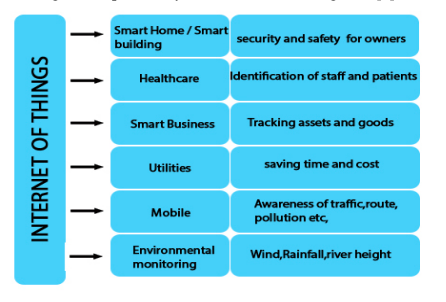
\includegraphics[width=3in]{Applications.png}
	\caption{\label{Applications}  Applications in IoT  , image source: 
		Principle Application and Vision in Internet
		of Things (IoT)\cite{App} }
\end{figure}

\section{Home Automation}

Since the late 70s, the concept of home automation has been taking place. With the increase of technology, people start to expect more of what home automation should provide and how the services will be done. This service has changed over time. The home automation system has always tried to provide a convenient, safe, and efficient way for homeowners to access their houses; despite that, the way to provide that is improved, but the system has remained the same.  


From an engineering point of view, Brand\cite{brand} specified a home after breaking it down into the "6 S's", Site, Structure, Skin, Services, space plan, and Stuff. Home automation systems will mainly concern with the last "3 S's, namely Service, Space Plan, and Stuff. A  modern home relies on three to seven services supported by companies like the Internet, gas, electricity, etc. Service provided plays a big role when defining home automation. As an example, the access to wireless communication helped with the "Space Plan" and improved the way how the modern home is like. In addition, homeowners can add or remove tools and equipment in their houses as they wish under the name of "Stuff."

\subsection{Challenges face home Automation }

 In his article \cite{Greichen}John J. Greichen  mentioned some of the early challenges faced by home automation systems, and they include : 
 
 
 \begin{itemize}
 	\item High manufacturing \& installation costs.
 \item Additional service and support costs.
 \item lack of home automation standards.
 \item Consumer unfamiliarity with the technology \& complex user interfaces. 
 	
 \end{itemize}

Over time, the development has grown very fast that led to a decrease in device size and price, and people are now familiar with using a computer, mobiles, and Laptops. Recently, using a wireless system like controlling devices via remote control or even wireless technology provided more advantages like reducing the installation costs since there is no cabling needed. Furthermore, internet connectivity allows us to control devices from any place via the mobile, and homeowners can add or remove devices easily and built-in the home automation system. 


 
 \subsection{Different Methodologies }
 
Bluetooth-based home automation system, which R.Piyare proposed and M.Tazil \cite{Tazil} , based on using a  smartphone, any microcontroller board, and Bluetooth technology offered a  secured and low-cost automation system. In this system, the communication between the board and mobile phone is done wirelessly using Bluetooth technology. Through the software application, the user will control the home appliances added to the system. To overcome the security issues and offer a high degree of protection, the system is used a password to allow only authorized users. A disadvantage to this system is the limitation to control the home appliances, as it is only covered within the Bluetooth range. Fig \ref{Blutooth} shows a block diagram of Bluetooth based home automation system. 

\begin{figure}[h!]
	\centering
	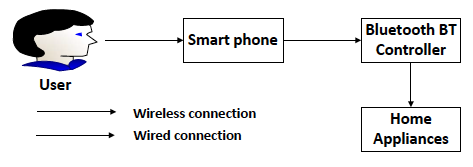
\includegraphics[width=3in]{Blutooth.png}
	\caption{\label{Blutooth}  Block diagram of home automation system 
		 , image source: An Overview of Home Automation Systems
		\cite{blutooth} }
\end{figure}


Another methodology is voice recognition-based home automation. The architecture hardware is also a microcontroller and smartphone, using Bluetooth technology to communicate. The new feature is offered via the mobile OS, which has a  built-in voice recognizing, which will allow the user to control the home appliances via voice command. The application transfers the user voice command into text, transmitted via Bluetooth to the microcontroller. A user only needs to pronounce the appliance name in the smartphone microphone and tell it to switch ON or OFF, which will ease the disabled and older people's ability to control all home appliances with no single move. The drawback is that it is not working efficiently in a noisy environment. Figure \ref {voice} shows the block diagram of a voice recognition-based home automation system. 



\begin{figure}[h!]
	\centering
	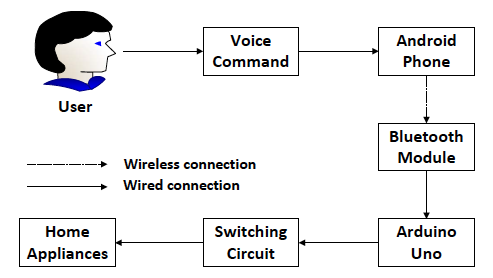
\includegraphics[width=3in]{voice.png}
	\caption{\label{voice}  Block diagram of voice recognition-based home automation
		, image source: An Overview of Home Automation Systems
		\cite{blutooth} }
\end{figure}

A real-life application using voice recognition in the home automation space is the smart-home controller Amazon Alexa. It can control several smart appliances and interact with several manufacturers using user's voice .lately; Amazon announced that Alexa can now pair with a Ring doorbell Pro and greet visitors and leave instructions about where to deliver packages.\cite{alexa}.


\subsection{Use Case: Smart Plugs}

As a use case to turn home to smart home allowing home automation concept, a smart plug is an electrical device that can be plugged into an ordinary outlet that can turn wired appliances into a controlled device in which the user will be able to control it by a mobile phone or voice command from anywhere. It is designed to connect the plug to the Wi-Fi home network. As a second step, the user needs to install the plug Application on his smart device to be able to control the electronic device plugged into the smart plug over the Internet. \cite{plug}. 

\begin{figure}[h!]
	\centering
	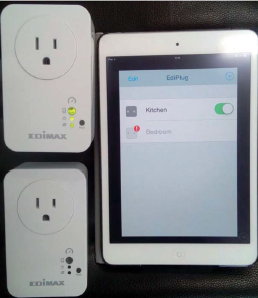
\includegraphics[width=2.5in]{plug.png}
	\caption{\label{plug}  Edimax plug and iPad installed with the control application.
		, image source: A Case Study of the Smart Plug System
		\cite{plug} }
\end{figure}

As an example of a smart plug Fig .\ref{plug} shows  Edimax SP-2101W smart plug connected with iPad as a controller tool. The plug can also help manage the energy consumption by allowing the user to observe the power usage. Moreover, the user can set a schedule with the time of turning on and off the device. The user needs to enter a username and password to assure more safety and security to access the plug and the attached device. Another feature is the user can add the email address and mobile number so that the plug can send an SOS message or email to alert the user in critical situations. 


\section{Building  Automation }

Traditionally, building automation starts with controlling electrical, mechanical, and plumbing systems within the building,e.g., heating, ventilation, air-conditioning, HVAC systems, lightning,  Close circuit video (CCTV), Fire alarm system...etc. Considering HVAC systems as the primary energy consumer in any building, operating and controlling these systems will affect the energy and cost.

\subsection{Building's Control Systems}

Before 1980 the control system was pneumatic based; despite that, it had some limitations to cover and control all the HVAC systems, it was widely used in a majority of existing buildings. By the 80s started the Analog electronic control devices spread, as they gave faster response and accurate results than pneumatics. In the 90s, the digital control device came on the market, then the whole function automation system was possible; what was not possible was mixing products from different vendors and manufacturers as they were not capable. The late 90s solved this issue as the were too many efforts to standardize one communication protocol. Finally, the American Society of Heating, Refrigerating and Air-conditioning Engineers (ASHRAE) implemented t the BACnet communication protocol, which became the industry open standard.\cite{control}

 Nowadays, the need to improve the operation and control of HVAC systems; most buildings are equipped with wide building automation systems (BASs) and building energy management control systems (EMCSs) to provide indoor comfort and a healthy environment and allow the automatic control of indoor conditions. In addition, the main aim of building automation systems is to achieve maximum savings in Energy and reduce the cost of maintenance by allowing access to all building services within the system.

The building's automation system is mainly hardware devices attached to devices or laying underfloor or even in the ceiling, where some customize control can be made. From a central management point of view, the BAS resides as software on an operator workstation (computer) or is available as a web page. Various types of "controllers" manage equipment and portions of the network. "Sensors" provide input data to the controllers.\cite{control}, The Fig. \ref{BAS} shows an overview of buildings' automation systems from soft and hardware perspectives. 



\begin{figure}[h!]
	\centering
	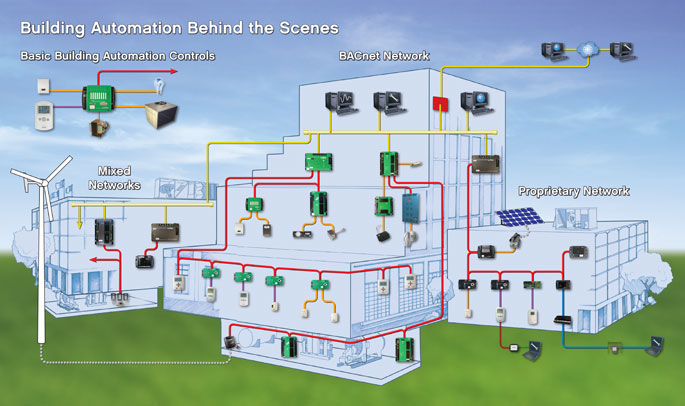
\includegraphics[width=3in]{BAS.png}
	\caption{\label{BAS}  Building automation system overview
		, image source: Understanding Building Automation and Control Systems
		\cite{control} }
\end{figure}

Furthermore, BMS systems extended to include controlling other outdoor functions like control and allowing the accessibility of the main building's door, the elevators and escalators control, security system, and fire detecting. 
 
 \subsection{IoT and buildings automation }
 

 The main aim of IoT technology is the integration of diverse physical objects into a global network, where all information about this object is presented on the internet, allowing interaction with and between this object ..Allowing access to the objects is already considered by the BAS concept by providing a virtual representation of this objects, e.g., sensors, control devices, actuators ...etc. BAS works within the local context of a functional building by linking both field tiers, sensors, and actuators, with an automation tire containing all control devices. The information then can be combined at the management tier. Fig . \ref{new }shows how BAS works. 

\begin{figure}[h!]
	\centering
	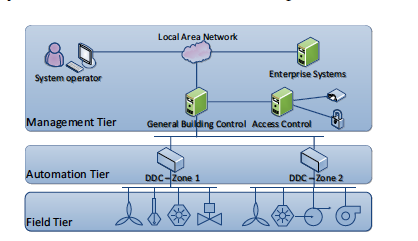
\includegraphics[width=2.5in]{newIOt.png}
	\caption{\label{new}  BAS  model
		, image source: Integrating Building Automation Systems and IPv6
in the Internet of Things
		\cite{NewIOT} }
\end{figure}



IoT's addition to the BAS system is crossing this local definition of borders since building automation already has a virtual representation on the Internet. It will then enable direct interaction with all things and services. When the building automation device is accessible on the Internet, that will add several features to building automation's traditional method. For example, considering the energy efficiency in the building, in functional building\cite{NewIOT}, energy can be saved by shifting energy consumption of HVAC devices to times when there is a lot of renewable energy available or when the electric grid is not overloaded. 


Having an energy-efficient solution and a friendly environment is one of the IoT goals to be achieved by applying smart building technology; integrating the IoT in building automation help in energy saving scenario. As an example\cite{NewIOT}, if we have a conference center, a building that includes many rooms and halls, which need to adjust the HVAC system according to its occupancy of it, other parameters can be added like the external temperature, Numbers of people in the room, and the sessions schedules at that time. To achieve better control of this building, we need to determine the exa exact occupancy of people in real-time and adjust the control parameters accordingly, including any change of schedule. Accessing all this data requires a global interaction on the internet via the cloud, which IoT can do. Applying this will save a massive amount of cooling and heating energy in the room that will not be occupied in this conference center. 


\subsection{Case study : Smart buldings}

Smart building is defined by The Institute for Building Efficiency \cite{smartB} \cite{mic}as the buildings that can provide low-cost services such as air conditioning, heating, ventilation, illumination, security, sanitation, and various other services to the tenants without adversely affecting the environment. For example, when the employees enter their company, the temperature, humidity, and lighting levels are edited to offer comfort and energy-saving conditions. In addition, it provides safety in case of any disasters like when there is a fire; the fire system can alert the ventilation system to turn off the fans to control the smoke and fire in a specific area.

To achieve this, we need to consider adding some intelligence from the design phase until the building is constructed. Using IT for interconnections between different systems in the buildings, sharing, storing, processing, and analyzing information will be possible. Fig . \ref{char}shows some characteristics and components
of a smart building. 



\begin{figure}[h!]
	\centering
	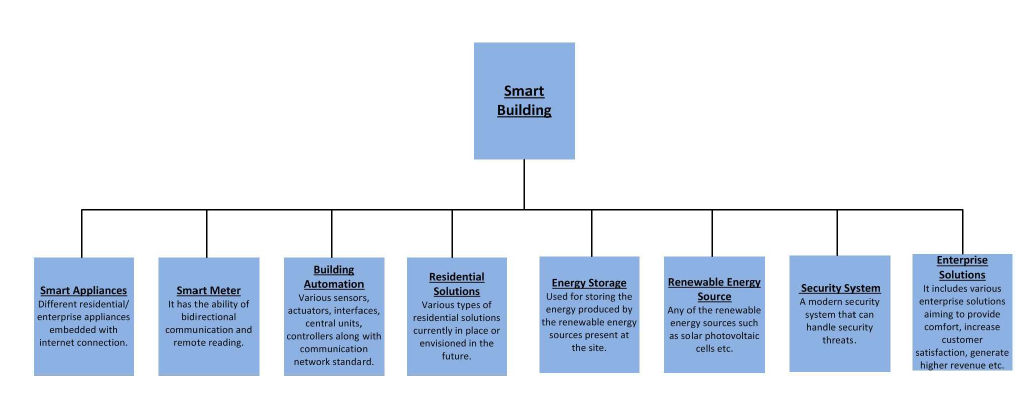
\includegraphics[width=3.5in]{charsb.png}
	\caption{\label{char}  characteristics and components
of a smart building
		, image source: Micro-location for Internet of Things equipped
Smart Buildings
		\cite{mic} }
\end{figure}


In order to handle all characteristics mentioned in Fig .\ref{char}, smart buildings require a high computational power, which a higher level of computing services can obtain. Cloud computing can implement this as it is reliable and allows the data to be accessible from anywhere. Cloud computing is used where dynamic resources are included as it offers a flexible and affordable way to manage IT resources. Those resources and services are needed to operate correctly. Hence, cloud computing is the way to process the data regarding resource use; it is also considered a place to store statistics and Information. \cite{frame}



\subsection{Challanges}

There are several
challenges that need to be addressed including the interoperability
of the devices, device smartness, security, privacy,
device energy consumption, device processing capability, and
network addressing \cite{mic}

\section{Evaluation \& Future work   }


\section{Conclusions  }



\begin{thebibliography}{00}
	
\bibitem{discovery}Zaslavsky, A., \& Jayaraman, P. P. (2015). Discovery in the Internet of Things. 
 
 \bibitem {RFID}D. Guinard, V. Trifa, and E. Wilde,( 2010) “A resource oriented architecture for the web of things,” in Proceedings of the 2nd International Internet of Things Conference (IoT ’10)
.
 \bibitem{SRA}Tarkoma, S., \& Katasonov, A. (2011). Internet of things strategic research agenda (IoT–SRA). Finnish Strategic Centre for Science, Technology, and Innovation: For Information and Communications (ICT) Services, Businesses, and Technologies, Finland.
 
 \bibitem{azori}Atzori, L., Iera, A., \& Morabito, G. (2010). The internet of things: A survey. Computer networks.
 
 \bibitem{App}Asghar, M. H., Negi, A., \& Mohammadzadeh, N. (2015, May). Principle application and vision in Internet of Things (IoT). In International Conference on Computing, Communication \& Automation .
 
 \bibitem{brand}Brand, S, How Buildings Learn, New York, Viking, 1994. 
 
 \bibitem{Greichen}Greichen, J.J., “Value based home automation or today's market,” IEEE Transactions on Consumer Electronics.
 
 \bibitem{Tazil}R. Piyare and M. Tazil, "Bluetooth based home automation system using cell phone," Consumer Electronics (ISCE), 2011 IEEE 15th
International Symposium on, Singapore.

\bibitem{blutooth} M. Asadullah and A. Raza, "An overview of home automation systems," 2016 2nd International Conference on Robotics and Artificial Intelligence (ICRAI).

\bibitem{alexa} Clark, Mitchell (February 11, 2021). "Alexa can now greet people from your Ring Doorbell Pro". theverge.com. Retrieved February 12, 2021.

\bibitem{plug}Ling, Z., Luo, J., Xu, Y., Gao, C., Wu, K., \& Fu, X. (2017). Security vulnerabilities of internet of things: A case study of the smart plug system. IEEE Internet of Things Journal.

\bibitem{control}KMC Controls.(May 2013) "Understanding Building Automation and Control Systems". 

\bibitem{NewIOT} Jung, M., Reinisch, C., \& Kastner, W. (2012, July). Integrating building automation systems and ipv6 in the internet of things. In 2012 Sixth International Conference on Innovative Mobile and Internet Services in Ubiquitous Computing (pp. 683-688). IEEE.


\bibitem{smartB}I. for Building Efficiency, “What is a Smart Building.” http://www.
institutebe.com/smart-grid-smart-building/What-is-a-Smart-Building.
aspx, 2008. [Online; accessed 02-Sept-2014].


\bibitem{mic}Zafari, F., Papapanagiotou, I., \& Christidis, K. (2015). Microlocation for internet-of-things-equipped smart buildings. IEEE Internet of Things Journal, 3(1), 96-112.


\bibitem{frame} Carrillo, E., Benitez, V., Mendoza, C., \& Pacheco, J. (2015, October). IoT framework for smart buildings with cloud computing. In 2015 IEEE First International Smart Cities Conference (ISC2) (pp. 1-6). IEEE.

\end{thebibliography}


\end{document}
